\documentclass[bibliography=totoc, paper=a4, fontsize=12pt]{scrreprt}
%fürs nächste mal nicht so große Abstände
\usepackage[left=2.5cm,right=2cm,top=1cm,bottom=1cm]{geometry}
\geometry{headheight=0.5cm, headsep=1.5cm, includehead}
\geometry{footskip=1.5cm ,includefoot}
\usepackage[ngerman]{babel}
\usepackage{caption}
\usepackage{booktabs}
\usepackage[colorlinks = true,
linkcolor =,
urlcolor  = blue,
citecolor = black,
anchorcolor = blue]{hyperref}
\usepackage{graphicx} 
\usepackage[headsepline,footsepline, automark, autooneside=false, markcase=used]{scrlayer-scrpage}
\pagestyle{scrheadings}
\usepackage{blindtext}
\usepackage{acronym}
\usepackage{enumitem}
\usepackage{tabularx}
\usepackage{enumitem}
\usepackage{ulem}
\usepackage[table]{xcolor}
\usepackage{xcolor,colortbl}
\usepackage{makecell} %for bigger lines in table
\usepackage{multicol}
\usepackage{multirow}
\usepackage{changepage}
\usepackage{ragged2e}
\usepackage{amssymb}
\usepackage{amsfonts} % <- zusätzliche Mathesymbole
\usepackage{mathtools} % <- zusätzliche Mathesymbole
\usepackage{setspace} %Zeilenabstand
\usepackage{pgfplots}
\usepackage{todonotes}
\usepackage{makecell}
\usepackage{lineno}
\usepackage{pdfpages}
\usepackage[parfill]{parskip} % <- delete all intents after paragraph
%%-----------------------------------------------------------------------------------
%% BibLaTex
\usepackage[backend=bibtex, style=numeric, sorting=none]{biblatex}
\addbibresource{source/quellen.bib}

%----------------------------------------------------------------------------------------
% 						Helping Commands
%
% \renewcommand{\arraystretch}{1.2} 	<- Tabelle strecken um 1.2 Punkte
% \rowcolors{1}{black!10}{black!1}		<- 
%

%Tabellenlinie
\newcommand\btrule[1]{\specialrule{#1}{0pt}{0pt}}

%Tabellenheader White & Bold
\newcommand{\whitebf}[1]{\color{white}\textbf{#1}}

%deutsche Anführungszeichen (german quote)
\newcommand{\gequote}[1]{\glqq #1\grqq{}}

%Auch bei chapter Header und Footer
\renewcommand*\chapterpagestyle{useheadings}

%Chapter Abstände
\renewcommand*\chapterheadstartvskip{\vspace*{-2.5\topskip}}
\renewcommand*\chapterheadendvskip{%
	\vspace*{1\baselineskip plus .1\baselineskip minus .167\baselineskip}}

\def\LayoutTextField#1#2{% label, field
	#2%
}
\renewcommand*{\DefaultOptionsofText}{print, bordercolor=black, borderstyle=U, backgroundcolor=blue!30}

\newcommand{\Todo}[1]{\todo[linecolor=red,backgroundcolor=red!25,bordercolor=red]{#1}}
\newcommand{\Info}[1]{\todo[linecolor=green,backgroundcolor=green!25,bordercolor=green]{#1}}

%\let\olditem\item
%\newcommand{\blueitem}{\color{blue}\olditem}
%\renewcommand{\item}{\color{black}\olditem}

\newcommand{\tablehead}[2]{\rowcolor{magicmint}\multicolumn{#1}{|c|}{#2}}
\newcommand{\foreign}[1]{\dashuline{#1}}

%tabularx Gimmick
\newcolumntype{R}{>{\raggedleft\arraybackslash}X}
\newcolumntype{L}{>{\raggedright\arraybackslash}X}
\newcolumntype{C}{>{\centering\arraybackslash}X}

%----------------------------------------------------------------------------------------
%	Listings
%----------------------------------------------------------------------------------------
\usepackage{listings}
\usepackage{color}

\definecolor{mygreen}{rgb}{0,0.6,0}
\definecolor{mygray}{rgb}{0.5,0.5,0.5}
\definecolor{mymauve}{rgb}{0.58,0,0.82}

\definecolor{black}{rgb}{0,0,0}
\definecolor{white}{rgb}{1,1,1}
\definecolor{magicmint}{rgb}{0.67, 0.94, 0.82}



\lstset{ 
	backgroundcolor=\color{white},   % choose the background color; you must add \usepackage{color} or \usepackage{xcolor}; should come as last argument
	basicstyle=\footnotesize,        % the size of the fonts that are used for the code
	breakatwhitespace=false,         % sets if automatic breaks should only happen at whitespace
	breaklines=true,                 % sets automatic line breaking
	captionpos=t,                    % sets the caption-position to bottom
	commentstyle=\color{mygreen},    % comment style
	deletekeywords={...},            % if you want to delete keywords from the given language
	escapeinside={\%*}{*)},          % if you want to add LaTeX within your code
	extendedchars=true,              % lets you use non-ASCII characters; for 8-bits encodings only, does not work with UTF-8
	firstnumber=1,                % start line enumeration with line 1000
	frame=single,	                   % adds a frame around the code
	keepspaces=true,                 % keeps spaces in text, useful for keeping indentation of code (possibly needs columns=flexible)
	keywordstyle=\color{blue},       % keyword style
	language=Octave,                 % the language of the code
	morekeywords={*,...},            % if you want to add more keywords to the set
	numbers=left,                    % where to put the line-numbers; possible values are (none, left, right)
	numbersep=8pt,                   % how far the line-numbers are from the code
	numberstyle=\footnotesize\color{mygray}, % the style that is used for the line-numbers
	rulecolor=\color{black},         % if not set, the frame-color may be changed on line-breaks within not-black text (e.g. comments (green here))
	showspaces=false,                % show spaces everywhere adding particular underscores; it overrides 'showstringspaces'
	showstringspaces=false,          % underline spaces within strings only
	showtabs=false,                  % show tabs within strings adding particular underscores
	stepnumber=1,                    % the step between two line-numbers. If it's 1, each line will be numbered
	stringstyle=\color{mymauve},     % string literal style
	tabsize=2,	                   % sets default tabsize to 2 spaces
	title=\lstname                   % show the filename of files included with \lstinputlisting; also try caption instead of title
}

\ihead{}
\chead{}
\ohead{\headmark}
%
\ifoot{}
\cfoot{\pagemark}
\ofoot{}

\begin{document}
\part{osm2inter}
\chapter{osm2pgsql}
\section{Intro}
Als Importierungskomponente kann osm2pgsql\cite{osm2pgsql-manual} sehr vielseitig eingesetzt werden. Innerhalb des Projektes löst osm2pgsql den OHDMConverter zum importieren von osm\textbar osm.pbf\textbar osm.bz2 in die intermediate Datenbank ab.\\

Den größten Vorteil von osm2pgsql bietet die Benutzung des \gequote{Flex Output}. Hierbei wird die Konvertierung mit einem lua Script angepasst.

\section{osm2pgsql Flags}
Für die fehlerfreie Importierung sind mehrere Flags notwendig. In der nachfolgenden \autoref{tb:flags} sind diese vermerkt.
\begin{table}[h]
	\caption{flags}
	\label{tb:flags}
	\renewcommand{\arraystretch}{1.5}
	\begin{tabularx}{\linewidth}{|l|X|}\hline
		Flag & Beschreibung\\\hline
		-c & Spezifiziert die osm Datei\\\hline
		-d & Name der Datenbank \\\hline
		-U & Name des Datenbankbenutzers mit Rechten zur Erstellung (Standard: postgres)\\\hline
		-O & Spezifiziert den Output z.B.: flex, pgsql (Standard), gazetteer und null\newline Für die Benutzung des lua Script basierten konvertierens, wird dieser Wert auf flex gesetzt\\\hline
		-x & Ermöglicht die Verwendung von user name, user id, changeset id, timestamp and version\\\hline
		-S & Dies gibt an, wie die Daten in die Datenbank importiert werden, ihr Format hängt von der Ausgabe ab\newline in diesem Flag muss das lua Script angegeben werden\\\hline		
	\end{tabularx}\vspace{0.5cm}
In Windows muss zusätzlich -W für eine Passworteingabe als Flag gesetzt werden
\end{table}

Ein Importierungsbefehl könnte nun wie folgt aussehen:
\begin{lstlisting}
	osm2pgsql -d ohdm -U postgres -O flex -x -S osm2inter.lua -c berlin.osm
\end{lstlisting}


\part{inter2ohdm}
\chapter{OHDM}
\section{Schema}
\begin{figure}[h]
	\caption{Schematischer Aufbau der OHDM Datenbank}
	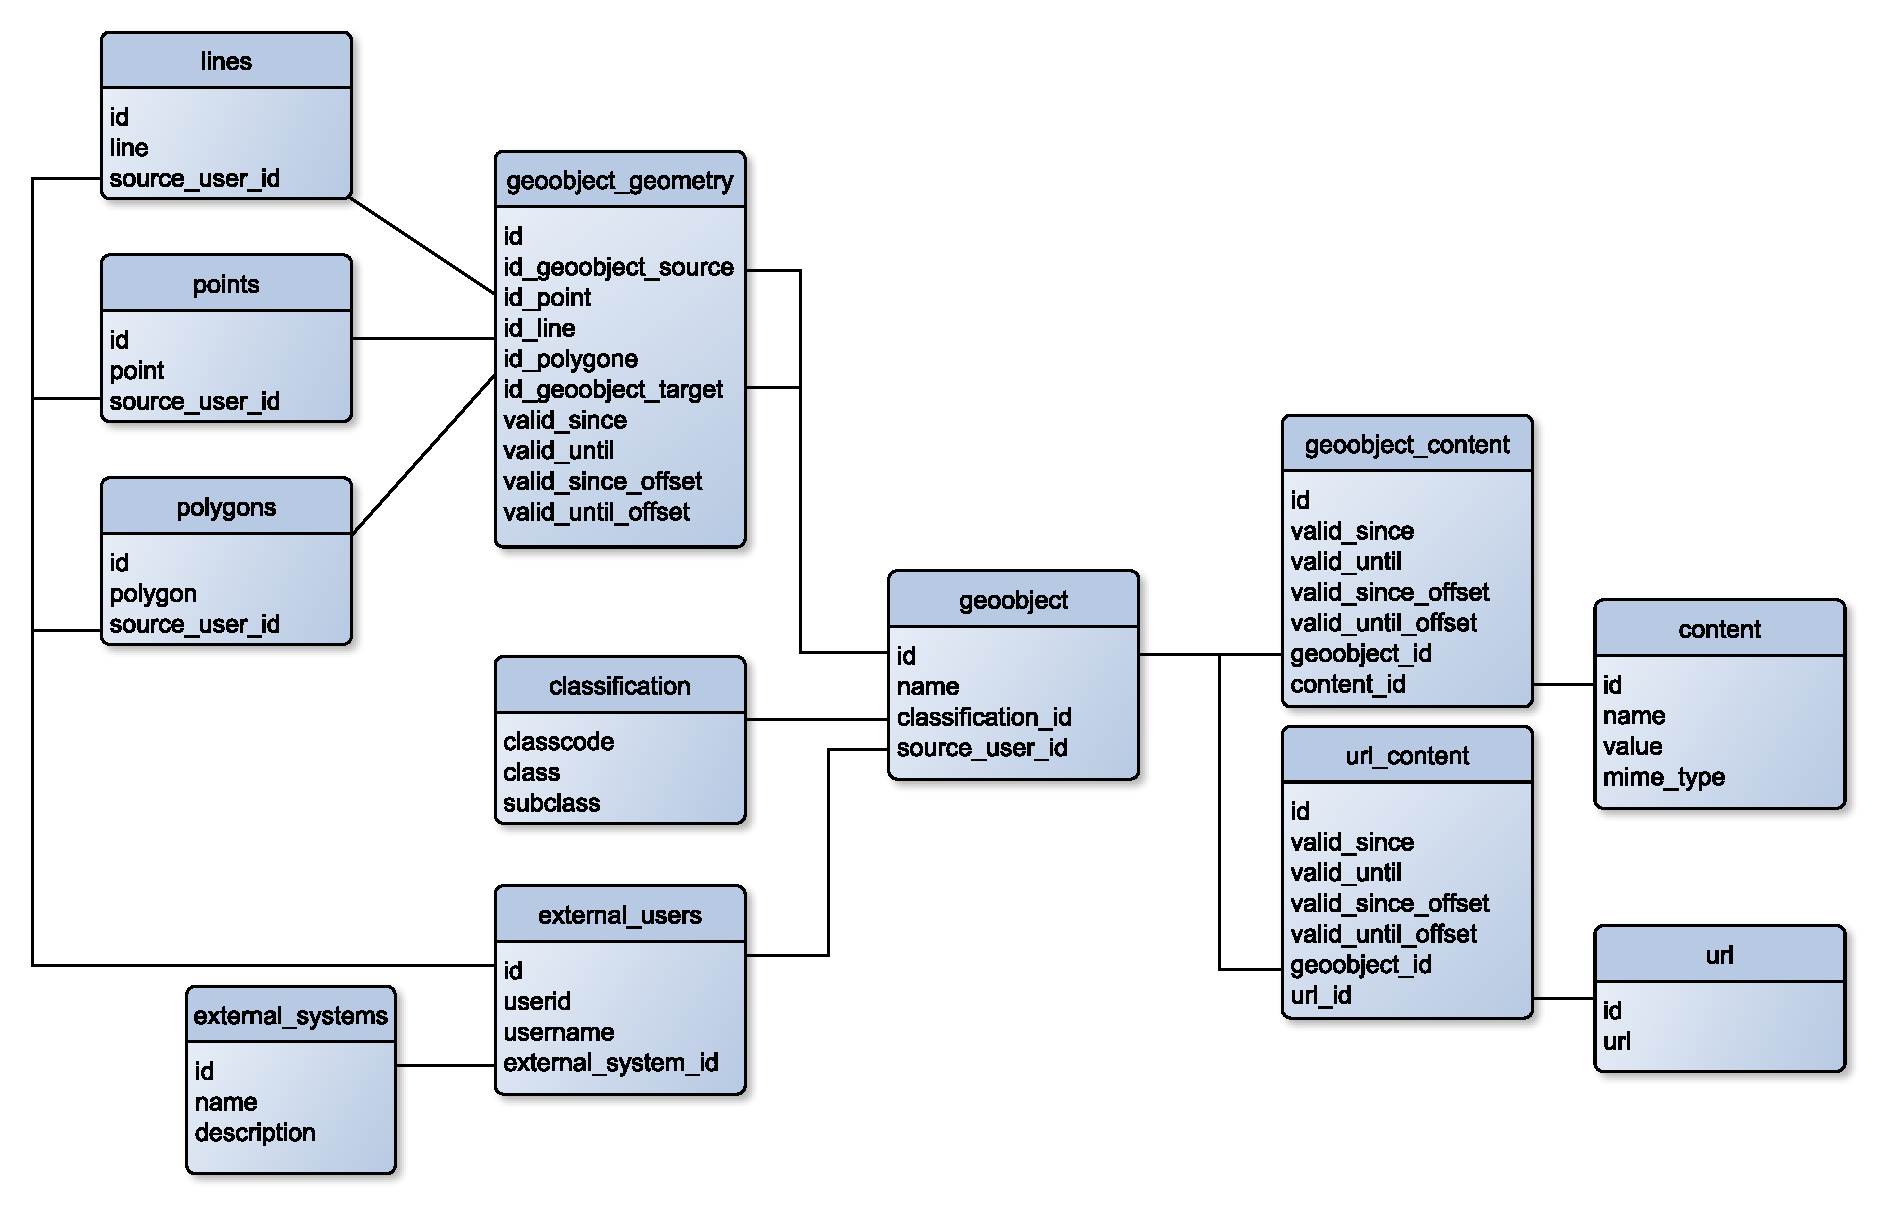
\includegraphics[width=\linewidth]{img/ohdm_datamodel.pdf}
\end{figure}
Die Erstellung des Schemas wurde mithilfe der existierenden Beschreibung von \\
\url{https://github.com/OpenHistoricalDataMap/OHDM-Documentation/wiki/OHDM-Data-Model} und den Konvertierten Einträgen des \gequote{alten} OHDMConverters realisiert.

\section{Theoretische Konvertierung}
\begin{figure}[h]
	\caption{Schematische Darstellung der einzelnen INSERT SQL Statemants}
	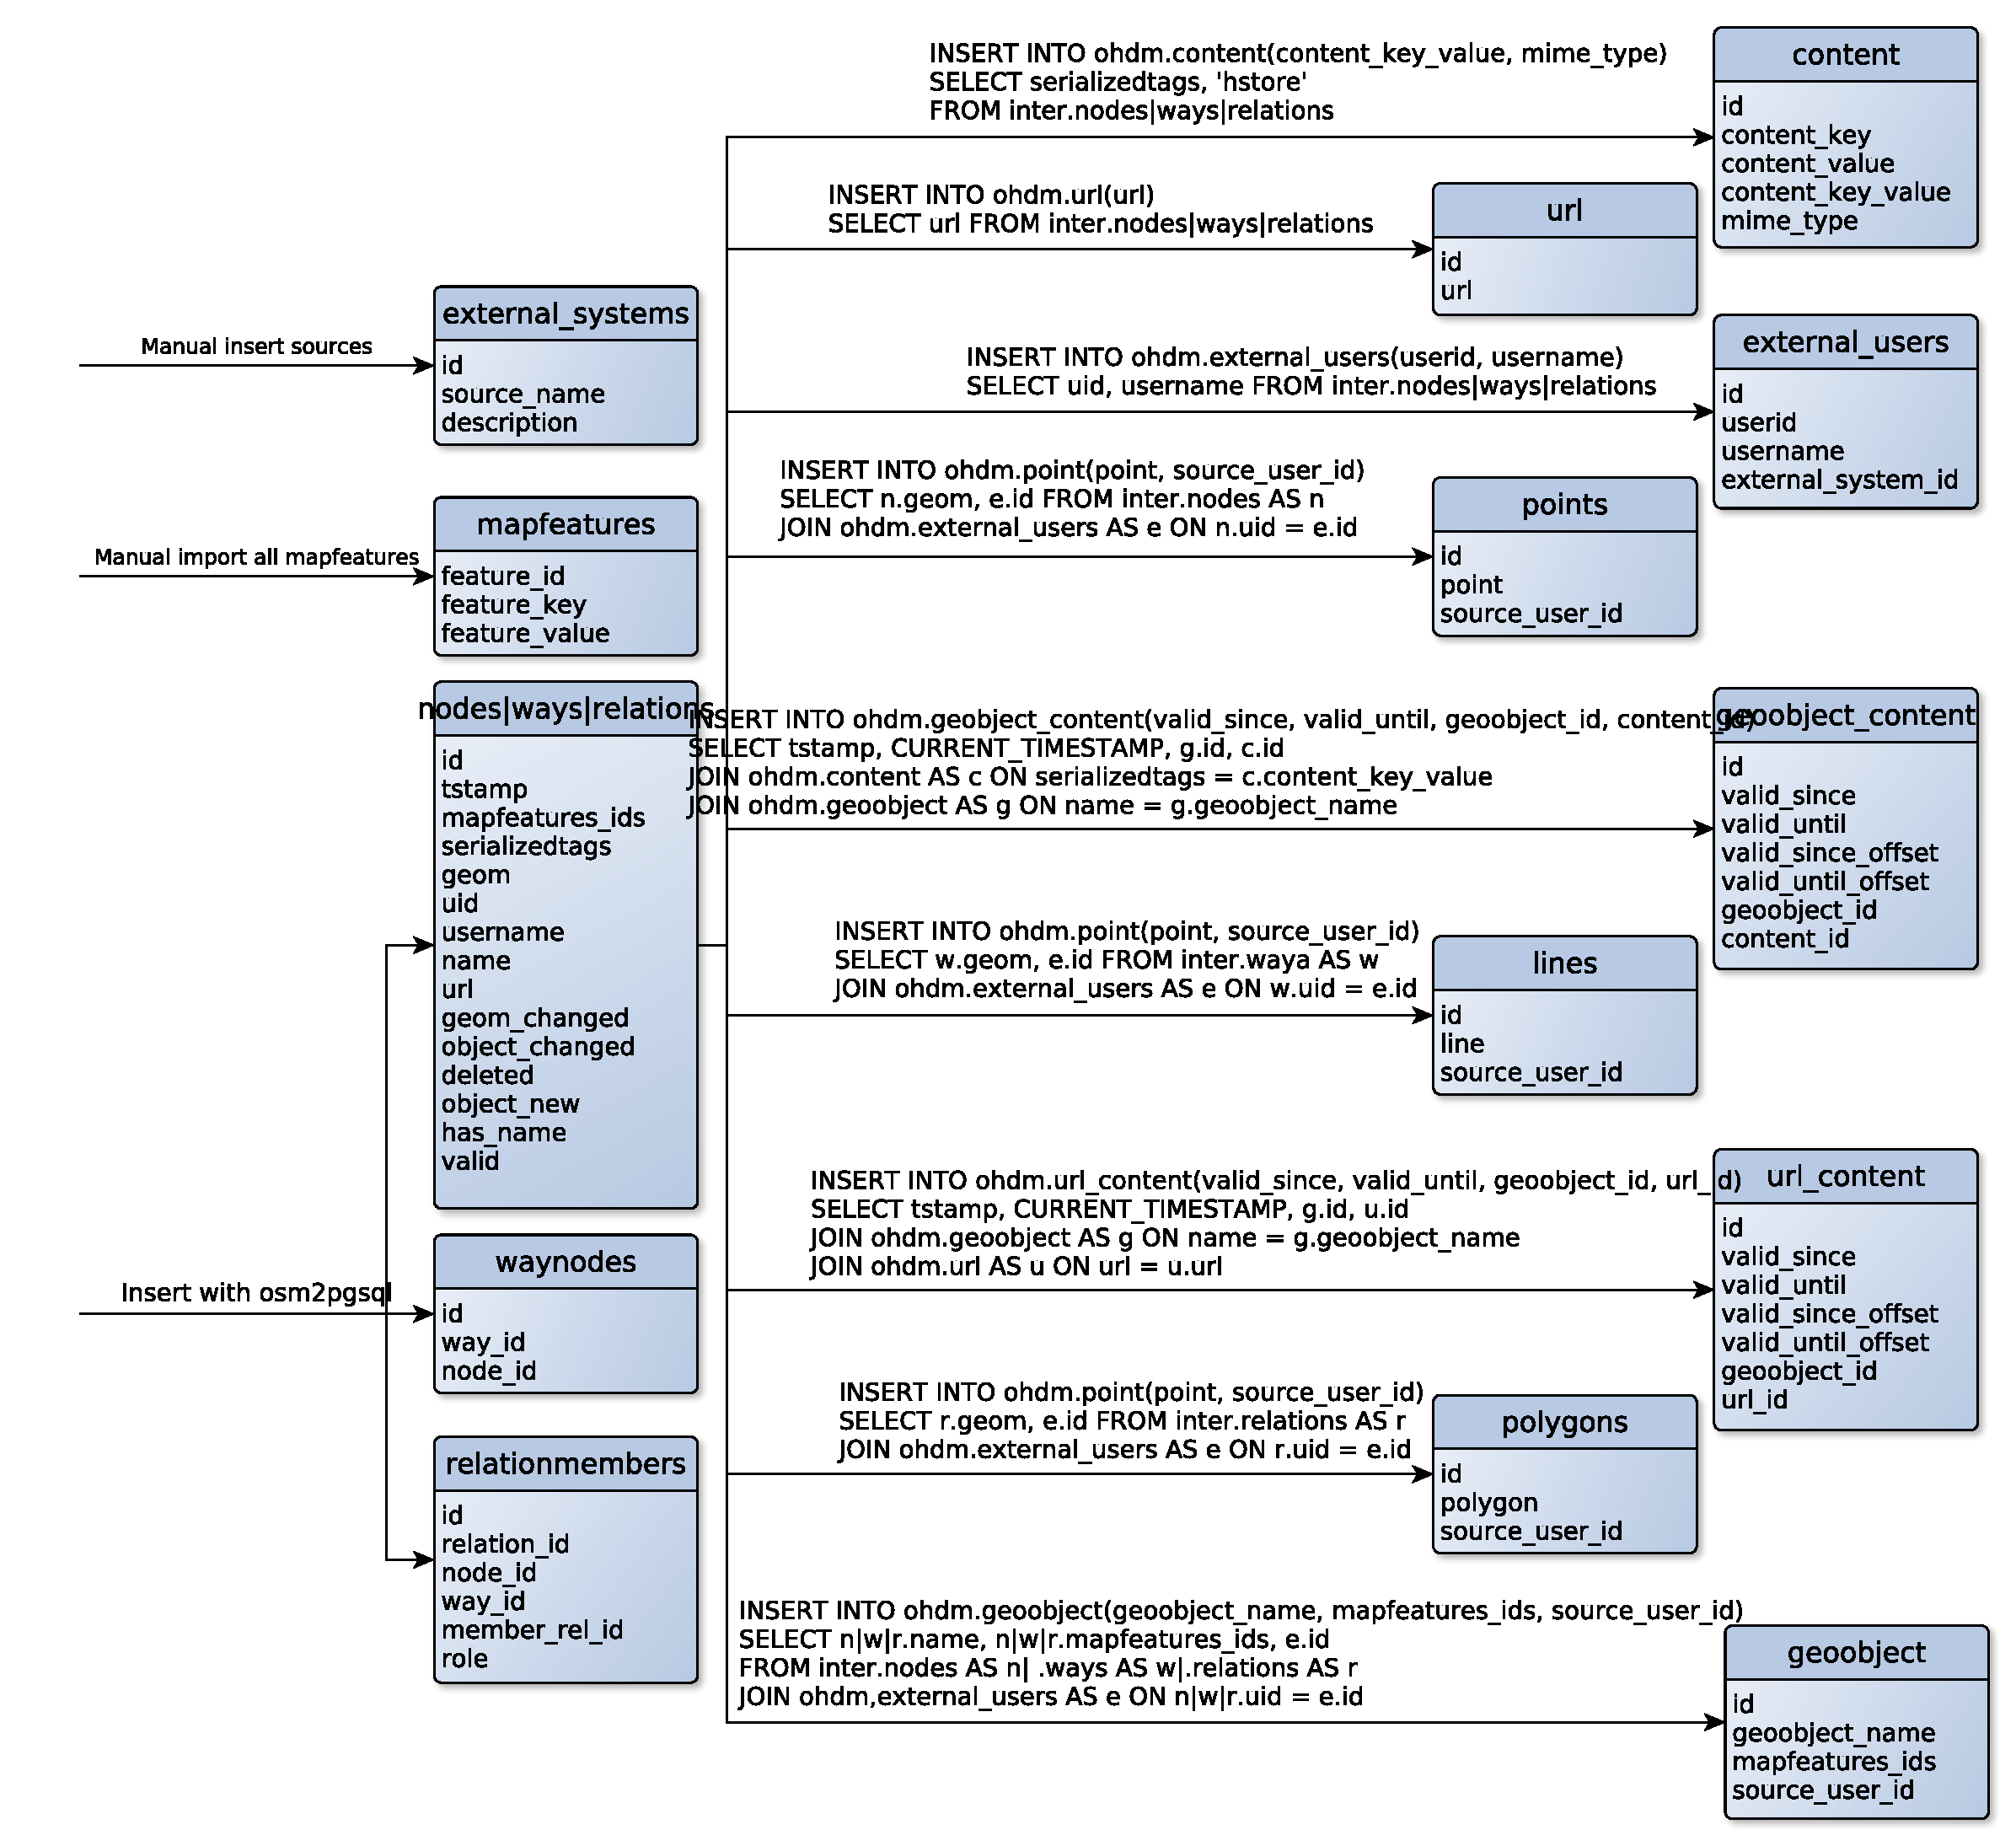
\includegraphics[width=\linewidth]{img/inter2ohdm_tableConvertionSchema1.pdf}
\end{figure}

\begin{figure}[h]
	\caption{Schematische Darstellung der einzelnen INSERT SQL Statemants}
	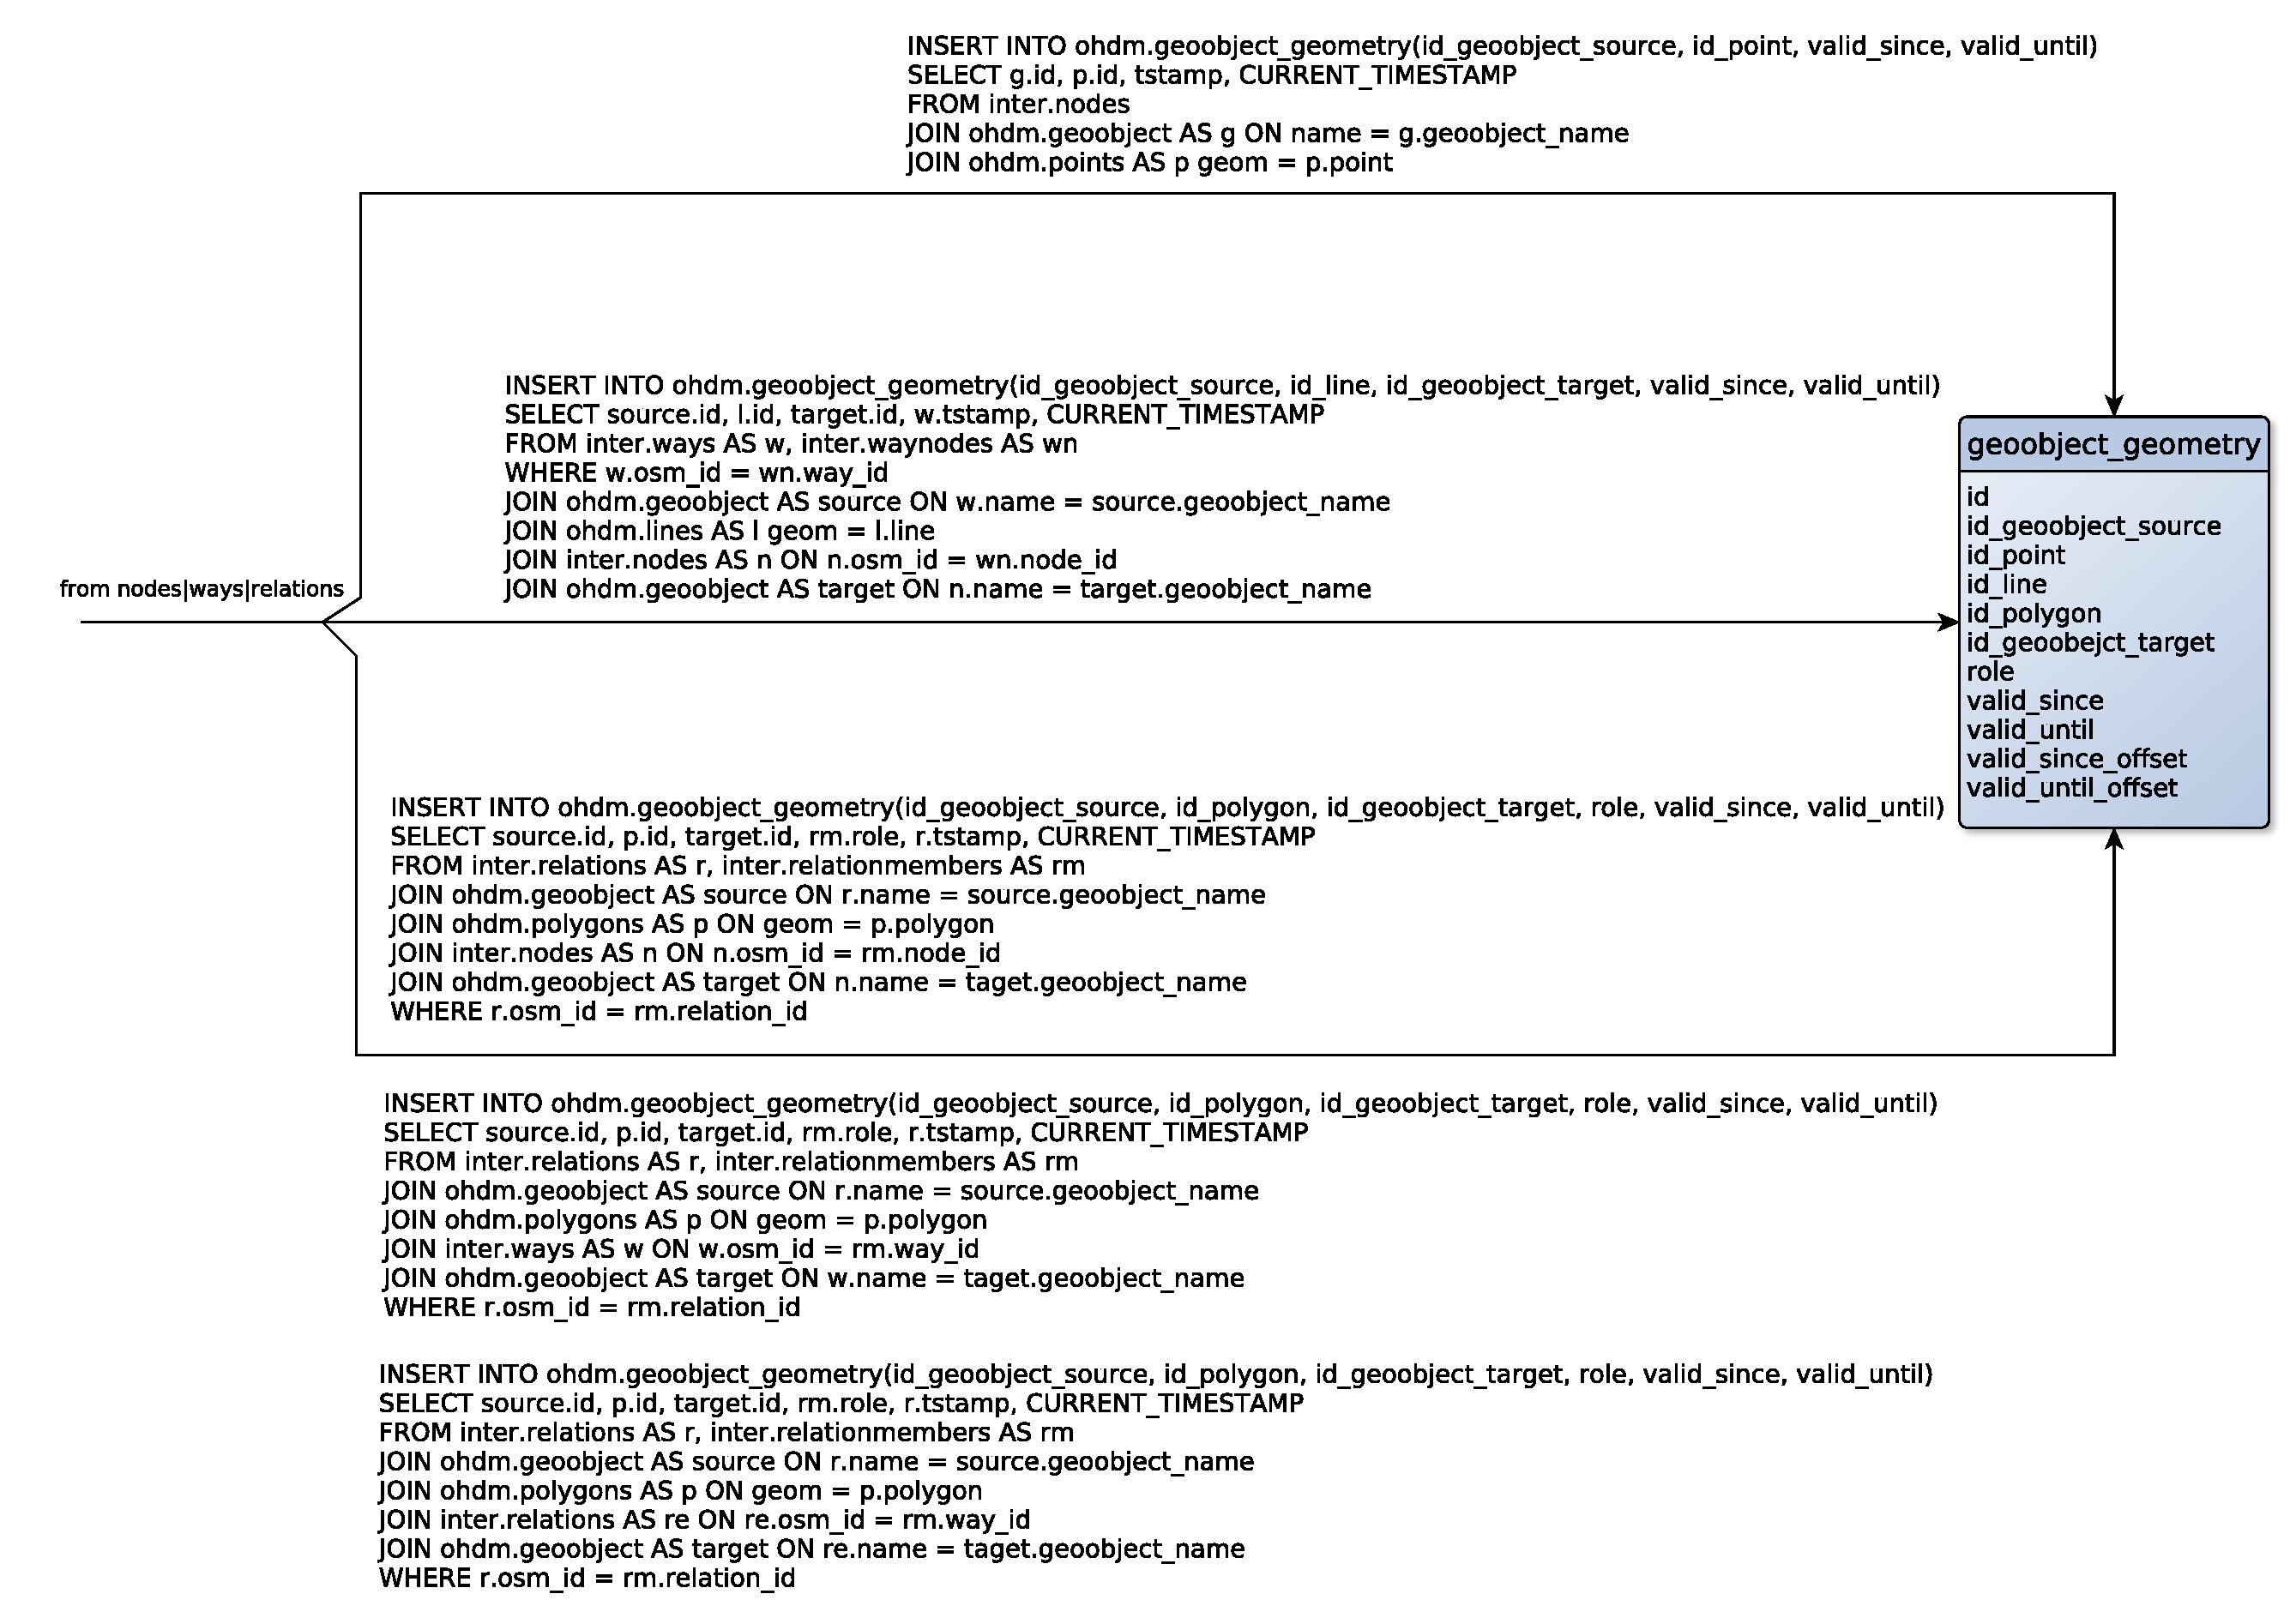
\includegraphics[width=\linewidth]{img/inter2ohdm_tableConvertionSchema2.pdf}
\end{figure}

\newpage
\clearscrheadings
\setheadsepline{0px}
\setfootsepline{0px}
\printbibliography[title={Quellenverzeichnis}]
\newpage
\setcounter{page}{1} \addtocontents{toc}{\protect\pagebreak}
\part{\appendixname}
\appendix
\ihead{} \chead{} \ohead{} \ifoot{} \cfoot{\pagemark} \ofoot{}

\newpage
\setheadsepline{.5px}
\setfootsepline{.5px}
\ohead{\headmark}
\chapter{Multiple Datenbanken in PostgreSQL}\label{ch:clustering}
Die Alternative zur Erstellung eines PostgreSQL Clusters ist die Verwendung von \lstinline[language=bash]|initdb|\cite{postgresql-cluster}, allerdings gibt mit dieser Variante einige Herausforderungen die mit \lstinline[language=bash]|pg_createcluster| leichter beziehungsweise überhaupt zu bewältigen waren.
\begin{enumerate}
	\item Steuerung des Clusters für die Serververwaltung
	\item Cluster als Service auch nach einem Neustart des Server starten
\end{enumerate}

\chapter{Windows Flag W}\label{ap:ch:win-pass}
Theoretisch sollte es möglich sein auch in Windows eine Peer Authentifizierung zuzulassen. Dafür müsste die Einstellung in der \lstinline|pg_hba.conf| geändert werden und dann validiert ob und wie mit der Datenbank interagiert werden kann.

\chapter{Curl Map Features}\label{ap:ch:curl-mapfeatures}
Um die Arbeit mit den Map Features\cite{osm-mapfeatures} zu erleichtern, müsste man ein curl Script implemntieren, dass die Tabelleneinträge auf der Map Features Webseite ausliest und in eine csv Datei oder ähliches schreibt.\\

\noindent Damit wäre es im Anschluss möglich die csv Datei als Insert Grundlage der classification Tabelle zu verweden.

\end{document}
